\chapter{Discussion}
Please tell more about conclusion and how to the next work of this study.

\section{Imron Sumadireja / 1164076}
\subsection{Teori}
\begin{enumerate}
\item Jelaskan kenapa file teks harus dilakukan tokenizer. Dilengkapi dengan ilustrasi atau gambar \par
Tokenizer merupakan proses membagi teks yang dapat berupa kalimat, paragraf atau dokumen menjadi kata-kata atau bagian-bagian tertentu dalam kalimat tersebut. Sebagai contoh dari kalimat `Aku mau istirahat dulu ya untuk hari ini', menjadi `Aku', `Mau', `'Istirahat',`Dulu',`Ya',`Untuk',`Hari',`Ini'. Yang menjadi acuan yakni tanda baca dan spasi. Untuk ilustrasinya bisa dilihat pada gambar \ref{toke1}
		\begin{figure}[!htbp]
		\centerline{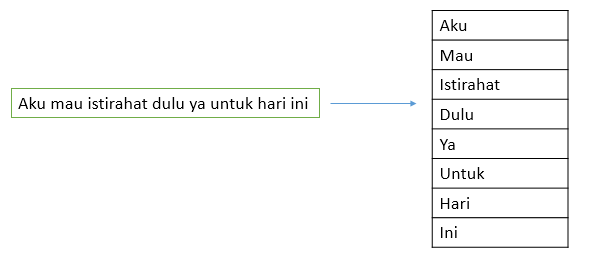
\includegraphics[width=0.5\textwidth]{figures/im/toke1.png}}
		\caption{Ilustrasi Tokenizer.}
		\label{toke1}
		\end{figure}

\end{enumerate}